\yesmargins

\chapter{Introduction}

\begin{tikzpicture}[overlay,remember picture] 
\node[anchor=south] at ([yshift=5in,xshift=0.6in]current page text area.south){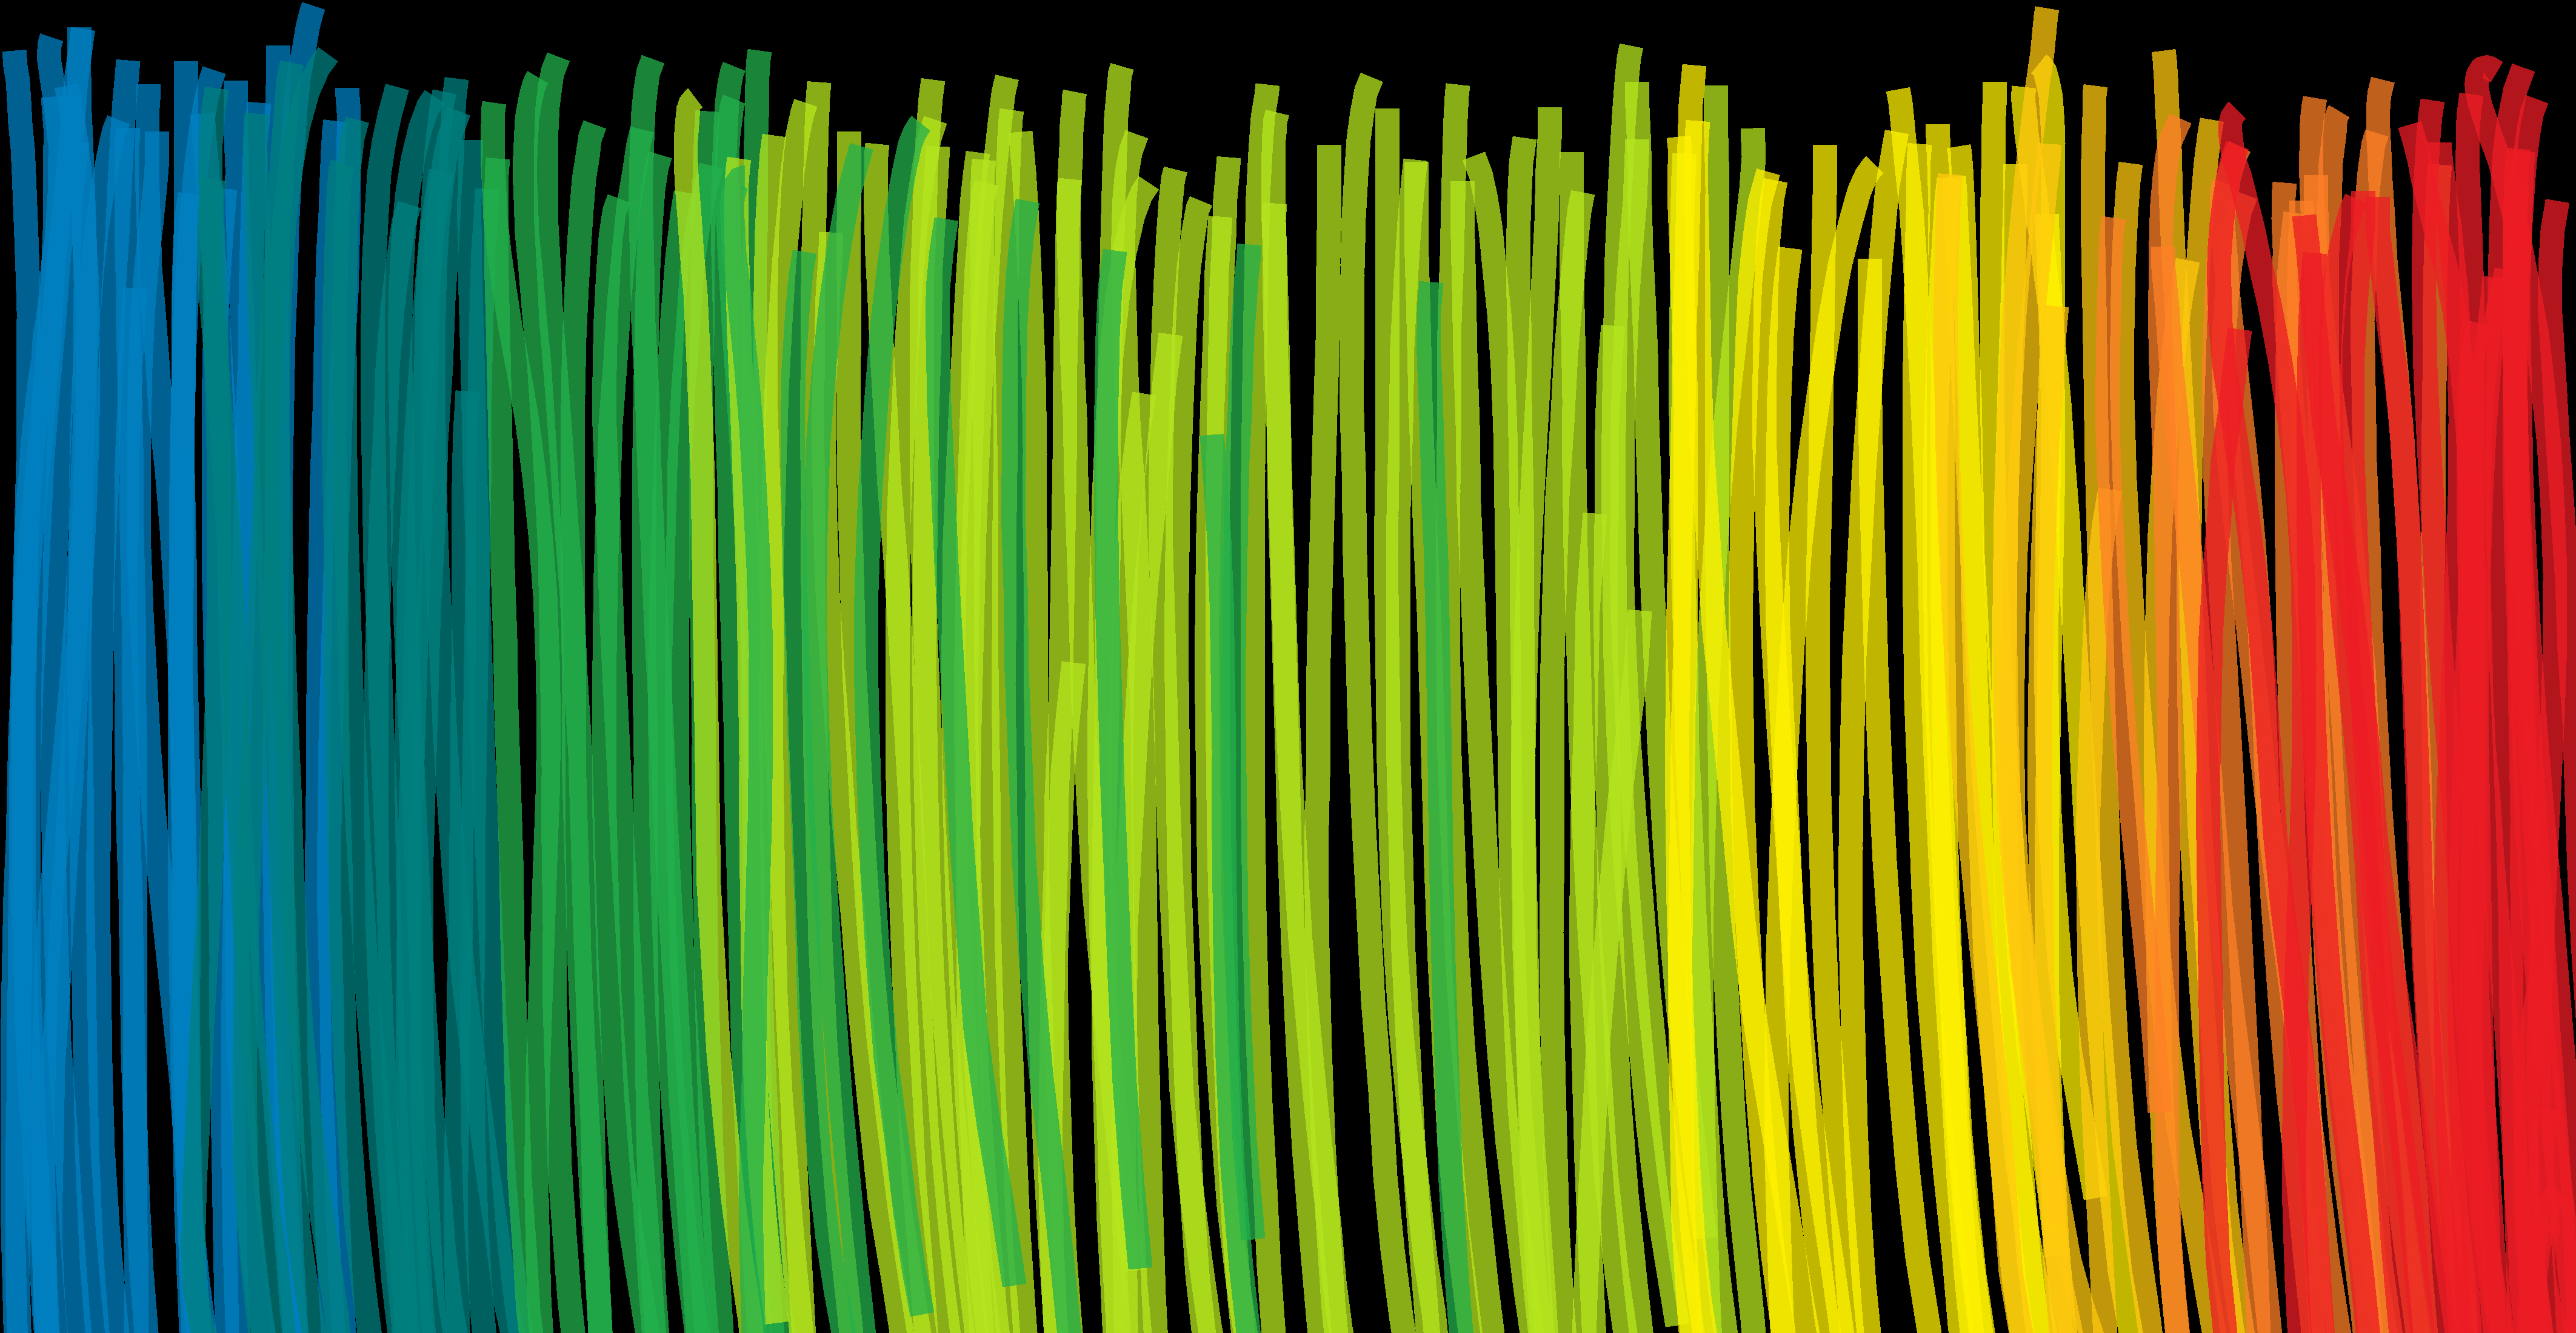
\includegraphics[width=10in]{intro}}; 
\end{tikzpicture} 

I won't tell you how to be a software engineer; You'll learn that over time by doing it. Instead, this book is about \textbf{software engineering methods}: Ways people achieve specific objectives in software engineering---that can save your project. My hope is that, after reading this book (or parts of it), you'll feel better equipped for software engineering.

\section{What's software engineering?}

Let's build a definition from the bottom up:\\

\begin{itemize}
\item Software engineering\index{software engineering} is \textbf{not} the same as \textbf{programming}
\item Software engineering involves trying to apply \textbf{methods}
\item Software engineering involves trying to make programs that have a long lifespan (\textbf{sustainable}\index{sustainability})
\item Software engineering involves trying to make programs that can be added to\marginpar{\methodDef\margindivider}\marginpar{\sustainabilityDef\margindivider}\marginpar{\extensibleDef\margindivider}\marginpar{\tripleConstraintDef\margindivider}\marginpar{\softwareEngineeringDef} (\textbf{extensible}\index{extensibility})
\item Software engineering involves trying to balance time, cost, and scope (the \textbf{triple constraint}\index{triple constraint})
\item Software engineering often involves \textbf{teamwork}\index{teamwork}
\item Software engineering involves trying to solve \textbf{problems people care about}
\item Software engineering involves both \textbf{artistry} and \textbf{science}.
\end{itemize}

\spacer
\textbf{Our definition:}

\begin{quote}
\textbf{Software engineering} is the art and science of using different methods to efficiently create extensible, sustainable programs that solve problems people care about.
\end{quote}

\section{What's the philosophy behind this book?}

My beliefs about software engineering influenced how I wrote this book. Some of my strongest beliefs about software engineering are described below.

\subsection{Software engineering is not black and white}
Throughout the book, I've tried to communicate that \textbf{software engineering is the gray area of computer science}. ``Right'' answers can be difficult to find and may not be reproducible in different contexts. Software engineering as a field also \textbf{keeps changing} as research scientists gather new findings, engineers develop new technologies, visionaries define new methods, and the outside world changes (e.g., a pandemic happened while I was writing this book and that changed how software engineering teams collaborate). Whereas in programming you might ask, ``Is this algorithm correct?'', questions in software engineering are more like, ``How does my team know this software is ready to release?'' or, ``People keep misinterpreting my code, how do I shift it toward better understandability\index{understandability} and maintainability\index{maintainability}?''

\subsection{Studying every detail of software engineering is a waste of time}\marginpar{\agileDef\margindivider}\marginpar{\softwareProcessModelDef\margindivider}\marginpar{\iterationDef\margindivider}\marginpar{\incrementDef}
I'm \textbf{not going to tell you everything} you need to know about software engineering because (1) what you need to know can be drastically different depending on \textbf{context} and (2) if I tried to, this book would be thousands of pages and possibly useless. Instead, I'll \textbf{introduce} a set of software engineering methods that are \textbf{known to be useful} across contexts, give guidance on when and why to use them, and point to \textbf{resources} for when you want more information.

\subsection{Agile isn't perfect but I really like it (and other people do too)}
This book leans so far toward \textbf{Agile} the two are probably in a relationship. That's because Agile development environments have become extremely \textbf{popular}---and because I like Agile: It matches how I think, and has been appropriate for nearly all the projects I've worked on. But you're not me, and Agile isn't the be-all-end-all, so I'm planning to incorporate more from other \textbf{software process models} in the future.

\section{What's this book like?}

It was \textbf{written iteratively} (``Do something. Now do it again, but better'') \textbf{and incrementally} (``Now do a little more''). Lots of software is written the same way. \\

\noindent It has \textbf{eight major topics}:\marginpar{Over here in the margin is where to find \textbf{definitions} (also in the Glossary).\margindivider}\marginpar{This is also where to find \textbf{asides}: Comments that are related to the content but don't fit into its flow or seem worth emphasizing.}

\begin{enumerate}
    \item \textbf{Agile}\index{agile}: Collaboration-oriented philosophy of creating software that values \textit{doing} over \textit{comprehensive planning} and \textit{documentation}
    \item \textbf{Project management \& teamwork}\index{project management}\index{teamwork}: Working in an organized way---and with other people
    \item \textbf{Requirements}: Being clear about what's expected of the software
    \item \textbf{Unified modeling language (UML) class and sequence diagrams}\index{UML}: A couple types of diagrams useful for communicating how your code works (or should work)
    \item \textbf{Monolith vs. microservices architectures}\index{monolith architecture}\index{microservices architecture}: Two contrasting high-level ways to organize code
    \item \textbf{Paper prototyping}\index{paper prototype}: Creating a good user interface design\index{user interface}\index{user interface design} before coding it
    \item \textbf{Cognitive style heuristics}\index{cognitive style heuristics}: Making software work well for different kinds of people who are not like you
    \item \textbf{Code smells \& refactoring}\index{code smells}\index{refactoring}: Making your code nicer to work with
\end{enumerate}

\noindent It's \textbf{short} and meant to be \textbf{readable}:\marginpar{This book might get shorter before it gets longer; I've tried to keep chapters concise but informative.}\\

\begin{itemize}
\item Important terms and concepts are \textbf{bolded}
\item Margins contain \textbf{term definitions} and side notes (relevant additional thoughts)
\item \textbf{Additional resources} are listed at the end of each major chapter\\
\end{itemize}

\textbf{My aim} is that you be able to quickly (1) determine whether each topic or method is \textbf{relevant} to your situation and (2) get a \textbf{basic understanding} of the topic or method so you can discuss it with others or have a starting point for exploring more.

\section{What's the future of this book?}

\marginpar{For \textbf{source files, updated versions, or to make suggestions}: \url{https://github.com/setextbook}}I'll keep iterating and incrementing. If you have content requests, suggestions, or other feedback, you can create an issue or pull request on this book's GitHub repository: \url{https://github.com/setextbook}. \\

\noindent \textbf{Potential future additions:}\\

\begin{itemize}
    \item Debugging
    \item Deployment
    \item DevOps
    \item Ethics
    \item More software architectures
    \item More software process models
    \item Object-oriented design principles
    \item Professionalism
    \item Software used by software engineers
    \item Testing your code (verification)
    \item More examples, figures, and images *\marginpar{* Yep, I'm the ``illustrator'' (a generous title).}
\end{itemize}

\spacer
This book could also become part of your own book / course / blog / etc.---feel free to use the whole thing or pieces of it (non-commercially).

\section{License}
Creative Commons Attribution-NonCommercial (CC BY-NC)

\section{Acknowledgments}
Thanks to Caius Brindescu, Raffaele de Amicis, S\`{e}anar Letaw, and Tiffany Rockwell for their feedback, advice, and support. Additional thanks to family and friends for their support. Thanks to the many software engineering students who gave feedback. Thanks to the Oregon State University Open Educational Resources Unit for making the whole effort possible.